\section{Pregibanje tangent na stožnice}
\label{pogl:stoznice}

Iz didaktičnega vidika zelo zanimivo poglavje nam predstavlja konstrukcije tangent na stožnice s prepogibanjem papirja. Vsebina je tu predstavljena tako, da je bralec najprej povabljen, da vzame list papirja in ga prepogiba po navedenih korakih. Po opažanju, kaj se na papirju pri tem prikaže, preidemo na matematični del, kjer dokažemo, da so prepogibi res tangente na določeno stožnico.

Učitelji matematike so povabljeni, da si pri obravnavi stožnic vzamejo čas in izvedejo spodnje aktivnosti. Dijaki bodo z veliko verjetnostjo presenečeni nad rezultati zgibanja, kar jih lahko bolj motivira za obravnavo geometričnih lastnosti stožnic. Priporočljiva je tudi izvedba ure v računalniški učilnici, kjer lahko vsak dijak z ustreznim programskim orodjem (npr.\ Geogebra) sam poskusi zgraditi opisano konstrukcijo. S tem lahko znanje o stožnicah le še bolj utrdi.

Z origamijem ne moremo konstruirati gladkih krožnih lokov. Kljub temu pa lahko z upoštevanjem določenih korakov konstruiramo premice, ki so tangentne na neko krivuljo. Več takih tangent nam poda nekakšno lomljenko, če pa bi konstrukcije pregibov ponavljali v nedogled, bi teoretično v limiti res dobili gladko krivuljo.

\begin{definicija}
    \label{def:ovojnica}
    Naj bo dana družina krivulj s parametrizacijo $F(t, x, y) = 0$, kjer je $t$ njen parameter in $F$ diferenciabilna za vsak $t$. \emph{Ovojnica} te družine je krivulja, ki je v vsaki točki tangentna na neko krivuljo iz družine. Dana je kot rešitev enačb
    $$ F(t, x, y) = 0 \; \text{ in } \; \frac{\partial}{\partial t} F(t, x, y) = 0. $$
\end{definicija}

\begin{opomba}
    Vsaka krivulja iz družine mora biti diferenciabilna in med krivuljami mora biti gladek prehod (\textcolor{red}{kako to bolj strokovno napisat?}). Vendar to ni zadosten pogoj, da ovojnica te družine družine obstaja -- protiprimer je družina krožnic s skupnim središčem in polmerom, ki se zvezno povečuje.
\end{opomba}

\begin{opomba}
    Ker so pregibi ravni, bodo v našem primeru krivulje v družini kar premice. Te premice so torej ravno tangente na ovojnico te družine.
\end{opomba}


\url{https://en.wikipedia.org/wiki/Envelope_%28mathematics%29}



Pa si poglejmo, kako s prepogibi dobimo tangente na vse štiri stožnice.

\subsection{Krožnica}

% Tega nikjer v literaturi ni in sem sama dodala. Malo preveč osnovno, ma če se obravnava tiste tri stožnice, pa se lahko kar vse, ane.

\textit{\textbf{Aktivnost:} Vzemi list papirja in svinčnik ter na sredi označi točko $S$. Nato drugje označi še točko $A$. Skozi točko $S$ prepogni poljubno premico in na njej označi točko $A'$, da velja $|SA| = |SA'|$. Nato skozi točko $A'$ prepogni pravokotnico na premico $SA'$. To je iskan pregib. To ponovi čimvečkrat za različno izbiro premice skozi točko $S$ (gl.\ sliko~\ref{fig:koraki_kroznica}). Kaj opaziš?}

\begin{figure}[h]
    \centering
    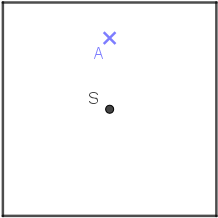
\includegraphics[width=0.3\textwidth]{images/stožnice/folding_kroznica_1.png}
    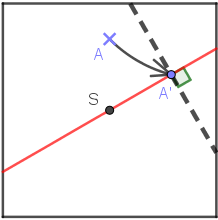
\includegraphics[width=0.3\textwidth]{images/stožnice/folding_kroznica_2.png}
    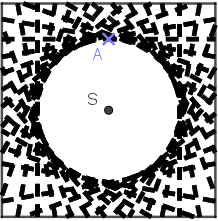
\includegraphics[width=0.3\textwidth]{images/stožnice/folding_kroznica_3.png}
    \caption[Prepogibanje krožnice]{Sukanje izbrane točke okoli središča.}
    \label{fig:koraki_kroznica}
\end{figure}

\opomba{V podpoglavju~\ref{zrcaljenje_origami} smo se naučili prenašati razdalje, zato je zgornja konstrukcija mogoča, zahteva pa še nekaj dodatnih vmesnih pregibov (gl.\ dokaz trditve~\ref{trd:prenasanje_razdalj}).}

Iz konstrukcije pregiba kot pravokotnice na premico $SA'$ skozi točko $A'$ je naslednja trditev očitna in ne potrebuje zapisanega dokaza.

\begin{trditev}
    Konstrukcija iz zgornje aktivnosti nam poda pregib, ki je tangenten na krožnico s središčem v točki $S$ in polmerom $SA$.
\end{trditev}

Za različno izbiro premic skozi točko $S$ dobimo različne tangente. S ponavljanjem konstrukcije tangente v neskončnost dobimo družino tangent, katere ovojnica je krožnica s središčem v točki $S$ in polmerom $SA$.

\subsection{Parabola}

\textit{\textbf{Aktivnost:} Vzemi pravokoten list papirja in svinčnik ter nekje sredi spodnje polovice lista s pisalom označi točko. Nato si izberi točko še na spodnji stranici lista in ga prepogni tako, da se obe izbrani točki prekrijeta. To ponovi čimvečkrat za različno izbiro točke na spodnji stranici papirja (gl.\ sliko~\ref{fig:koraki_parabola}). Kaj opaziš?}

\begin{figure}[h]
    \centering
    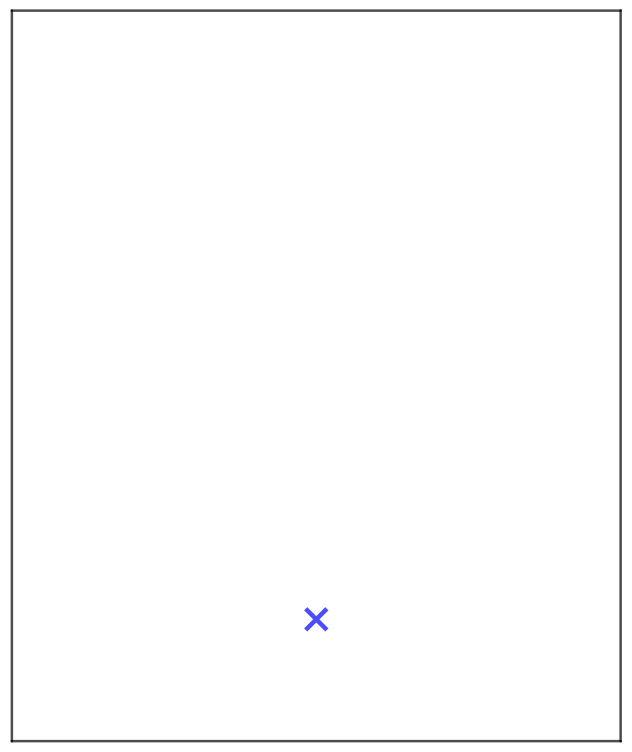
\includegraphics[width=0.3\textwidth]{images/stožnice/folding_parabola_1.png}
    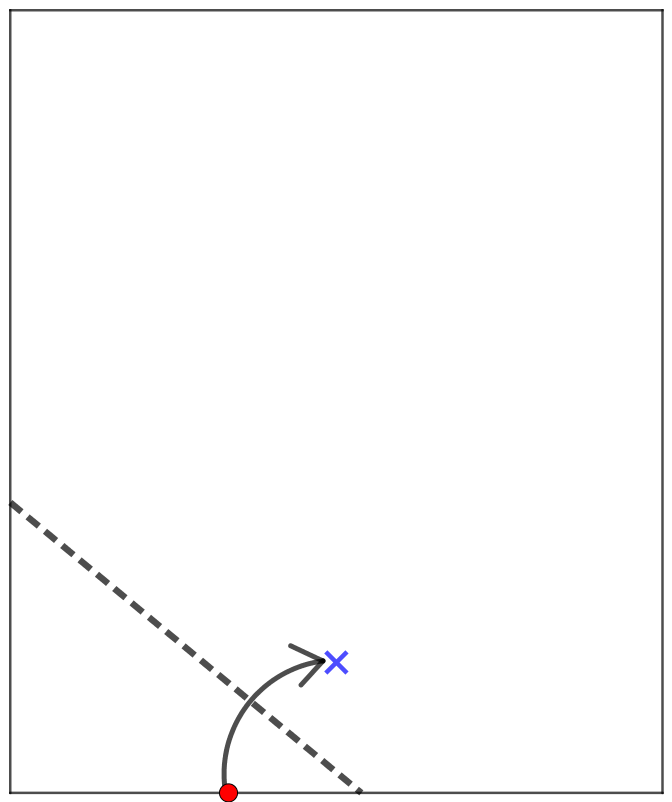
\includegraphics[width=0.3\textwidth]{images/stožnice/folding_parabola_2.png}
    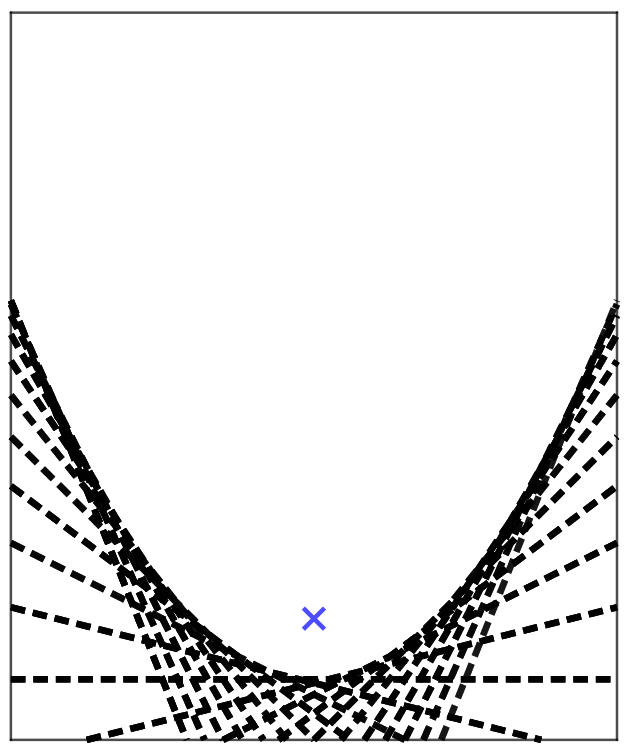
\includegraphics[width=0.3\textwidth]{images/stožnice/folding_parabola_3.png}
    \caption[Prepogibanje parabole]{Prepogibanje spodnje stranice papirja na izbrano točko.}
    \label{fig:koraki_parabola}
\end{figure}

% Najstareši opis zgornje konstrukcije, ker sem jih našla, je v svojo knjigo \emph{Geometric Exercises in Paper Folding} vključil indijski matematik T.\ Sundara Row~\cite{row1917}.
% Hull je našel Row-a (prvič izdana 1893) kot najstarejši zapis te konstrukcije

Omenjen pregib je origami operacija~\ref{op:O3}, lahko pa nanjo gledamo tudi kot na operacijo~\ref{op:O6}. Za le-to smo v poglavju~\ref{pogl:aksiomi} že premislili, da nam pregib, ki poteka skozi dano točko $B$ in točko $A$ položi na premica $a$, poda tangento na parabolo z goriščem $A$ in premico vodnico $a$ (gl.\ sliko~\ref{fig:O6_parabola} in premislek nad njo). Tukaj pa take točke $B$ ni, kar pomeni le to, da smo s pregibom konstruirali neko tangento -- pregib je namreč simetrala daljice, ki ima za krajišči obe izbrani točki iz navodila aktivnosti, torej obstaja točka (točka $P$ na sliki~\ref{fig:O6_parabola}), ki je enako oddaljena od spodnje stranice lista in prve izbrane točke. Nadaljni premislek, da je to edino presečišče pregiba in parabole, je enak kot prej. Spodnja trditev je tako že dokazana.

\begin{trditev}
    Konstrukcija iz zgornje aktivnosti nam poda pregib, ki je tangenten na parabolo z goriščem v izbrani točk in premico vodnico, ki jo predstavlja spodnja stranica lista.
\end{trditev}

Ker je vsak pregib tangenten na isto parabolo, je obris, ki bi nastal po neskončno pregibih, res ta parabola.

To je bil intuitiven premislek. Poglejmo si, kako lahko to dokažemo na bolj matematični način.

Začnimo kar s parametrizacijo družine konstruiranih pregibov. V ta namen v model poljubne točke in spodnje stranice lista vpeljimo nekaj oznak. Naj bo $c \in \mathcal{O}$. Vzemimo točko $A(0, c)$ in premico $a: y = -c$, ki sta origami-konstruktibilni, in naredimo pregib, ki točko $A$ preslika na premico $a$ v točko $A'(t, -c)$ za nek $t \in \R$ (slika~\ref{fig:enacba_tangente_par1} v primeru $c = 1$).

\begin{figure}[h]
    \centering
    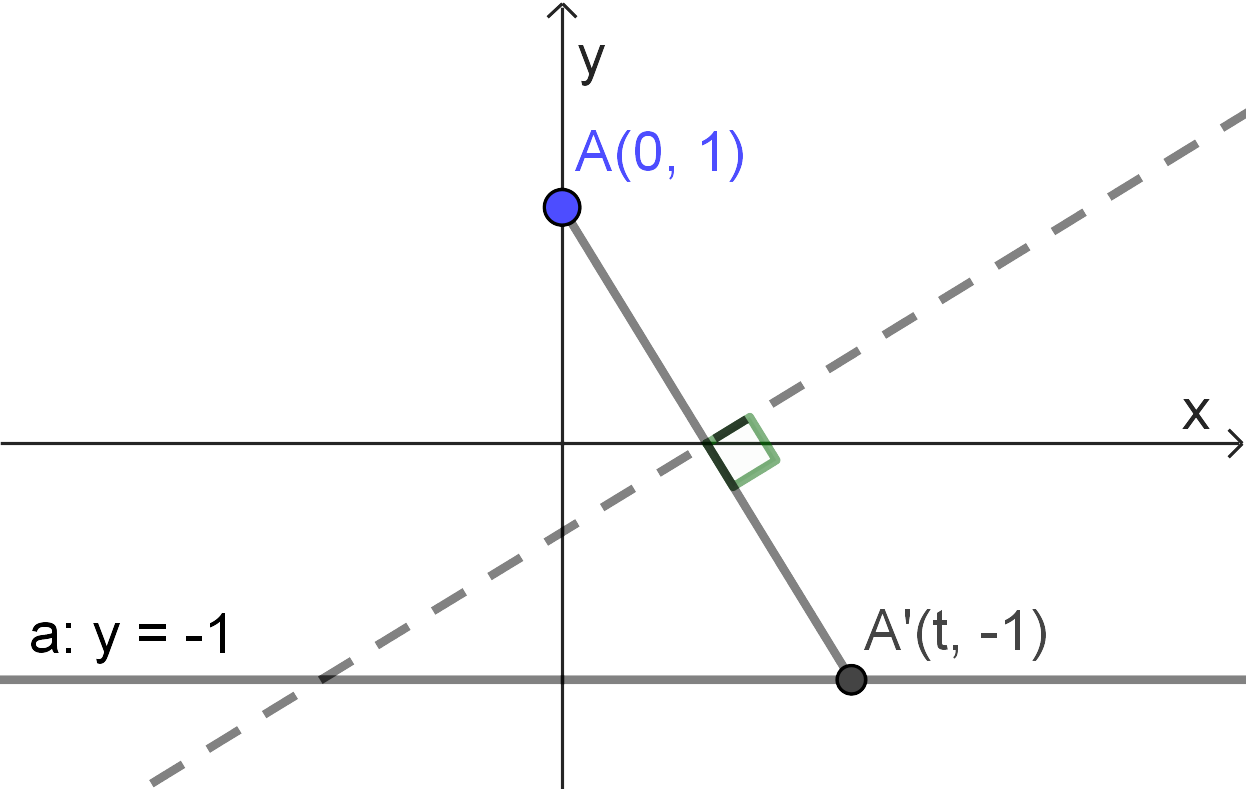
\includegraphics[width=0.5\textwidth]{images/enacba_parabole1.png}
    \caption[Enačba tangente na parabolo]{Pregib točke $A(0, 1)$ na premico $a: y = -1$ (primer za $c = 1$).}
    \label{fig:enacba_tangente_par1}
\end{figure}

Ker je pregib oz.\ konstruirana premica simetrala daljice $AA'$, lahko hitro določimo njeno enačbo. Koeficient nosilke daljice $AA'$ je $k_A = -\frac{2c}{t}$, središče pa $(\frac{t}{2}, 0)$. Tako hitro določimo enačbo pregiba:
\begin{equation}
    y = \frac{t}{2c} x - \frac{t^2}{4c}.
    \label{eq:tang_par}
\end{equation}
Dobili smo iskano parametrizacijo družine pregibov z enačbo
$$F(t, x, y) = \frac{t}{2c} x - y - \frac{t^2}{4c} = 0. $$
Za vsak $t \in \R$ torej dobimo drugo tangento na parabolo z goriščem v točki $A$ in premico vodnico $a$ z zgornjo enačbo~\ref{eq:tang_par}. Izrazimo sedaj enačbo ovojnice preko sistema enačb iz definicije~\ref{def:ovojnica}. Iz enačbe $(\partial / \partial t) F(t, x, y) = 0$ dobimo $x/(2c) - 0 - (2t)/(4c) = 0$ oz.\ $x = t$. Ko to vstavimo v enačbo $F(t, x, y) = 0$, dobimo
\begin{equation}
    \label{eq:parabola_splosna}
    y = \frac{x^2}{4c},
\end{equation}
torej je ovojnica res parabola. Njeno enačbo lahko dobimo tudi brez definicije ovojnice. Ker so vse točke na pregibu enako oddaljene od točk $A$ in $A'$, na pregibu obstaja le ena točka $T$, za katero velja $d(T, A) = d(T, a)$. Njena abscisa je $x = t$ (točka $T$ leži na pregibu točno nad točko $A'$) in iz enačbe~\ref{eq:tang_par}, dobimo še ordinato $y = t^2/(4c)$. Ker točka $T$ za vsak $t \in \R$ leži na paraboli, pri menjavi $x = t$ dobimo ravno enačbo~\ref{eq:parabola_splosna}.

Preden gremo na naslednji način dokaza, si poglejmo še vpliv parametra $c$ na parabolo. Razdalja med njenim goriščem in premico vodnico je $2c$ in iz enačbe~\ref{eq:parabola_splosna} je razvidno, da bo z manjšanjem $c$ parabola vedno ožja.

Hull v~\cite[str.\ 55--56]{hull2013} poda prefinjen dokaz preko kvadratne formule. Vemo, da pregib~\ref{op:O6} ne obstaja vedno (slika~\ref{fig:O6} desno). Poglejmo, ali obstajajo v ravnini našega modela kakšne točke, skozi katere ne moremo konstruirati pregiba oz.\ tangente. Vzemimo našo parametrizacijo družine tangent (enačba~\ref{eq:tang_par}) in za lažje reševanje privzemimo $c = 1$. Če jo rešimo za $t$, nam dobljena formula pove, za katere vrednosti $t$ pregib poteka skozi točko $(x, y)$:
$$ \frac{1}{4}t^2 - \frac{x}{2}t + y = 0 \Rightarrow t_{1,2} = \frac{\frac{x}{2} \pm \sqrt{\frac{x^2}{4} - y}}{\frac{1}{2}}.$$
Enačba ima dve realni rešitvi pri pogoju $x^2 / 4 - y > 0$, kar pomeni, da vsako točko $(x, y)$, za katero ta pogoj velja, sekata dva pregiba. To so ravno točke pod parabolo $y = x^2 / 4$. Za točke \emph{na} paraboli velja $y = x^2 / 4$, iz česar dobimo eno rešitev $t = x$, torej to točko seka natanko en pregib. Nazadnje nam ostane še območje, za katerega velja $y > x^2 / 4$, t.\ j.\ območje nad parabolo $y = x^2 / 4$, kar nam ne poda realnih rešitev za $t$, torej ga ne seka noben izmed konstruiranih pregibov. Tako je obris, ki ga dobimo v nalogi, res parabola $y = x^2 / 4$.

Aktivnosti za naslednji dve podpoglavji sta enaki kot v tem, le da namesto spodnje tranice lista v izbrano točko prepogibamo krožnico.

\subsection{Elipsa}

\textit{\textbf{Aktivnost:} Vzemi list papirja in svinčnik ter na sredini nariši poljubno krožnico. Označi njeno središče. Na notranji strani krožnice si izberi poljubno točko. Izberi si točko na krožnici in list prepogni tako, da se obe izbrani točki prekrijeta. To ponovi čimvečkrat za različno izbiro točke na krožnici (gl.\ sliko~\ref{fig:koraki_elipsa}). Kaj opaziš?}

\begin{figure}[h]
    \centering
    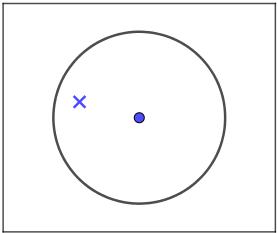
\includegraphics[width=0.3\textwidth]{images/stožnice/folding_elipsa_1.png}
    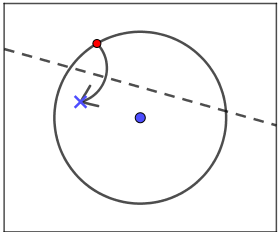
\includegraphics[width=0.3\textwidth]{images/stožnice/folding_elipsa_2.png}
    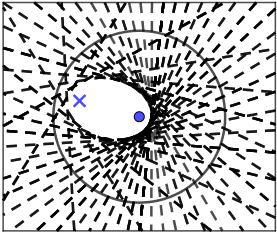
\includegraphics[width=0.3\textwidth]{images/stožnice/folding_elipsa_3.png}
    \caption[Prepogibanje elipse]{Prepogibanje krožnice na izbrano točko znotraj nje.}
    \label{fig:koraki_elipsa}
\end{figure}

\opomba{Za izris poljubne krožnice tu lahko uporabimo šestilo. Prej smo videli, da znamo lomljeno krožnico prepogniti tudi z origamijem, vendar imamo potem na listu papirja veliko pregibov, ki nam ovirajo pogled na ciljno sliko. Zato je uporaba šestila v ta namen dovoljena predvsem iz praktičnega vidika.}

Izgleda, kot da se nam izriše elipsa, ki ima za gorišči središče krožnice in izbrano točko znotraj nje. Spomnimo se, da na elipsi ležijo vse točke, katerih vsota razdalj do obeh gorišč je konstantna in enaka dolžini velike osi (t.\ j.\ dvakratnik velike polosi). V našem primeru je elipsa natančno določena, kar nam pove naslednja trditev~\cite[str.\ 60--61]{hull2013}.

\begin{trditev}
    Konstrukcija iz zgornje aktivnosti nam poda pregib, ki je tangenten na elipso z goriščema v obeh izbranih točkah in veliko osjo, enako polmeru izbrane krožnice.
\end{trditev}

\begin{dokaz}
    Naj bo točka $F_1$ središče krožnice s polmerom $r$ in točka $F_2$ poljubna točka znotraj krožnice. Potem je elipsa, ki ima ti dve točki za svoji gorišči in veliko os enako $r$, natančno določena. Po navodilih iz aktivnosti konstruiramo en pregib, pri čemer na krožnici izberemo poljubno točko $A$ (slika~\ref{fig:dokaz_elipsa} levo). Dokazujemo, da je tangenten na to elipso.

    Označimo s $T$ presečišče pregiba in daljice $AF_1$ (slika~\ref{fig:dokaz_elipsa} desno). \textcolor{red}{(Ali presečišče vedno obstaja? Ja, samo še dokaži to)} Ker je pregib simetrala daljice $AF_2$, velja $|TA| = |TF_2|$, torej je
    $$|TF_1| + |TF_2| = |TF_1| + |TA| = |F_1A| = r$$
    za vsako izbiro točke $A$. Ker je $r$ velika os elipse, točka $T$ leži na njej.

    Pokažimo še, da je pregib tangenten na elipso. Opazimo, da so vsi trije koti z vrhom v točki $T$, ki imajo za enega od krakov pregib, skladni. Značilnost tangent na elipso pa je ravno ta, da se žarek, ki ga izstrelimo iz enega gorišča v rob elipse, vedno pod istim kotom odbije v drugo gorišče.
    \begin{figure}[h]
        \centering
        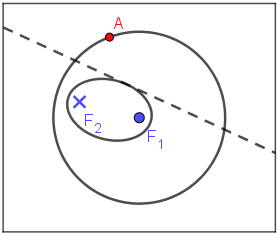
\includegraphics[width=0.3\textwidth]{images/stožnice/elipsa_dokaz1.png}
        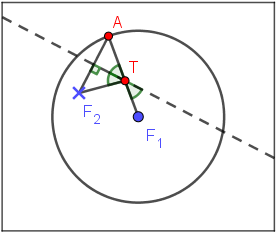
\includegraphics[width=0.3\textwidth]{images/stožnice/elipsa_dokaz2.png}
        \caption[Tangentnost na elipso]{Dokaz tangentnosti pregibov na elipso.}
        \label{fig:dokaz_elipsa}
    \end{figure}
    Torej je pregib tangenten na dano elipso v točki $T$.
\end{dokaz}

\textcolor{red}{Bi se dalo dobit enačbo preko ovojnice?}

Kaj se zgodi, če točko izberemo \emph{zunaj} krožnice, pa si pogledamo v naslednjem razdelku.

\subsection{Hiperbola}

\textit{\textbf{Aktivnost:} Vzemi list papirja in svinčnik ter na sredini nariši poljubno krožnico. Označi njeno središče. Na zunanji strani krožnice si izberi poljubno točko. Izberi si točko na krožnici in list prepogni tako, da se obe izbrani točki prekrijeta. To ponovi čimvečkrat za različno izbiro točke na krožnici (gl.\ sliko~\ref{fig:koraki_hiperbola}). Kaj opaziš?}

\begin{figure}[h]
    \centering
    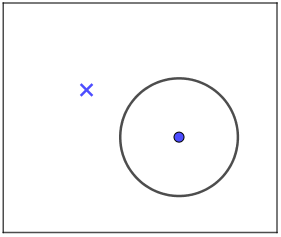
\includegraphics[width=0.3\textwidth]{images/stožnice/folding_hiperbola_1.png}
    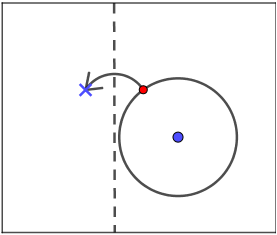
\includegraphics[width=0.3\textwidth]{images/stožnice/folding_hiperbola_2.png}
    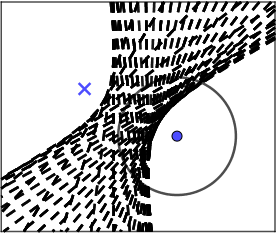
\includegraphics[width=0.3\textwidth]{images/stožnice/folding_hiperbola_3.png}
    \caption[Prepogibanje hiperbole]{Prepogibanje krožnice na izbrano točko zunaj nje.}
    \label{fig:koraki_hiperbola}
\end{figure}

Podobno kot prej lahko sklepamo, da se nam izriše obris hiperbole. Spomnimo se, da na hiperboli ležijo vse točke, katerih absolutna vrednost razlike razdalj do obeh gorišč je konstantna in enaka dolžini velike osi. Tako kot pri elipski je tudi tu hiperbola natančno določena. Naslednja trditev in dokaz sta zato zelo podobna kot za elipso.

\begin{trditev}
    Konstrukcija iz zgornje aktivnosti nam poda pregib, ki je tangenten na hiperbolo z goriščema v obeh izbranih točkah in veliko osjo (t.\ j.\ dvakratnik velike polosi), enako polmeru izbrane krožnice.
\end{trditev}

\begin{dokaz}
    Naj bo točka $F_1$ središče krožnice s polmerom $r$ in točka $F_2$ poljubna točka zunaj krožnice. Potem je hiperbola, ki ima ti dve točki za svoji gorišči in veliko os enako $r$, natančno določena. Po navodilih iz aktivnosti konstruiramo en pregib, pri čemer na krožnici izberemo poljubno točko $A$ (slika~\ref{fig:dokaz_hiperbola} levo). Dokazujemo, da je tangenten na to hiperbolo.

    Označimo s $T$ presečišče pregiba in nosilke daljice $AF_1$ (slika~\ref{fig:dokaz_hiperbola} desno). \textcolor{red}{(Ali presečišče vedno obstaja? NE, V 2 PRIMERIH DOBIMO ASIMPTOTO - ko je premica vzporedna k pregibu)} Ker je pregib simetrala daljice $AF_2$, velja $|TA| = |TF_2|$, torej je 
    $$\left||TF_1| - |TF_2|\right| = \left||TF_1| - |TA|\right| = |F_1A| = r$$
    za vsako izbiro točke $A$. Ker je $r$ velika os hiperbole, točka $T$ leži na njej.

    Pokažimo, da je to res tangenta. Ker je pregib simetrala daljice $F_2A$,  prepolavlja kot $\angle ATF_2$, ki je enak kotu $\angle F_1TF_2$. Torej pregib skozi točko T na hiperboli prepolavlja kot, ki ga ta točka oklepa z goriščema, to pa je ravno značilnost tangent na hiperbolo (\textcolor{red}{zase: pokazi de je to rejs}).

    \begin{figure}[h]
        \centering
        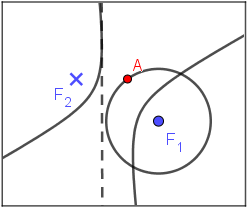
\includegraphics[width=0.3\textwidth]{images/stožnice/hiperbola_dokaz1.png}
        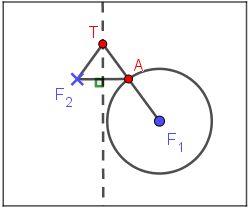
\includegraphics[width=0.3\textwidth]{images/stožnice/hiperbola_dokaz2.png}
        \caption[Tangentnost na hiperbolo]{Dokaz tangentnosti pregibov na hiperbolo.}
        \label{fig:dokaz_hiperbola}
    \end{figure}
    Torej je pregib tangenten na dano hiperbolo v točki $T$.
\end{dokaz}

\textcolor{red}{Bi se dalo dobit enačbo preko ovojnice?}

Bolj analitičen dokaz, kjer se izračuna splošno enačbo elipse in hiperbole glede na izbrano krožnico in točko znotraj oz.\ zunaj nje, najdemo v~\cite[str.\ 204--206]{smith2003}. Tudi Lotka v~\cite{lotka1907} iz opisane konstrukcije izpelje splošno enačbo elipse in tudi nastavi popravek, ki nam da splošno enačbo hiperbole. S tem oba dokažeta, da je ogrinjača teh pregibov res elipsa oz.\ hiperbola.
\textcolor{red}{Nekaj je tudi v~\cite[str.\ 34 spodaj]{hull2020}.}